
\section{Methodology}

Discrete mathematics and computer science often deal with different types of data abstractions and structures such as sets, trees, and graphs, where concepts like nodes and links are used to describe the topology a collection of objects and manipulate their data \citep[e.g.,][]{Skiena_2008_Book}. In graphs, the data---sometimes also referred to as the payload---resides at the vertices or nodes who are connected through links or edges, which may or may not have an associated direction. A visibility graph is a special type of undirected graphs in which the links are straight lines connecting intervisible nodes; that is, straight lines that do not overlap any obstacle while connecting nodes that can see each other in a physical space \citet{LozanoPerez_1979_CACM}. Visibility graphs have been mostly used in robotics for navigation path planning \citep[e.g.,][]{Huang_2004_Proc, Oommen_1987_JRA} but have also seen applications in other fields including urban studies, interior architecture, medicine and geosciences \citep[e.g.,][]{Raman_2010_UE, Ahmadlou_2010_JNT, Varoudis_2014_JSS, Phillips_2015_ESR}.

In a relatively recent study, \citet{Lacasa2008} applied the concepts of visibility graphs to the representation and analysis of time series. Multiple applications have been found to this idea in fields like economics \citep{Yang_2009_PA, Wang2012} and climate \citep{Elsner_2009_GRL}. In this study, we are particularly interested in the application of visibility graphs to the analysis of seismic sequences \citep{Telesca2012}. In this case, the nodes in the visibility graphs are considered to be seismic events distributed over time. For any seismic time series, two characteristics are attributed to each event: (a) its occurrence time, and (b) the value associated to the event, here considered as the magnitude. The obstacles in the time space are the vertical lines (or sticks) between the time axis and the magnitude of the event in a time-magnitude series. Two events are in connection, or visible to each other, whenever no other event interrupts their linear connection.

In mathematical form, events $i$ and $j$ are visible to each other if they satisfy the inequality
%
\begin{equation}
	\frac{y_i - y_p }{t_p - t_i} > \frac{y_i - y_j}{ t_j - t_i} \, ,
\end{equation}
%
\noindent
where $y$ is the value associated with the event and $t$ is the time of the event. The index $p$ indicates any event occurring between events $i$  and $j$. It follows from this that the visibility graph generated from a time series holds the following conditions. Connectivity: each event is visible to the immediate first events to its right and left sides, if there is any. Directivity: the graph is considered undirected by definition; that is, the algorithm explaining the connections between events is developed without defining a direction for the links between the events. And invariance: scaling or time-shifting the series does not change the resulting visibility graph, provided the transformation is done under affine conditions \citep{Lacasa2008}.

Figure \ref{fig:vg} shows an example of a visibility graph for one of the magnitude-time series to be considered later in this study. For each event $i$ we compute the connectivity degree, $k$, which is the sum of the connections to all other events $j$ visible by the $i$th event. Events are often categorized in small magnitude bins with $\Delta M = 0.1$ and we plot the connectivity degree as a function of the bin magnitude. Note that two earthquakes with the same magnitude can have different $k$ values, which ultimately depend on the occurrence time of the event and whether the time-neighboring events are of a larger or smaller magnitude.

\begin{figure*}[t]
	\centering
	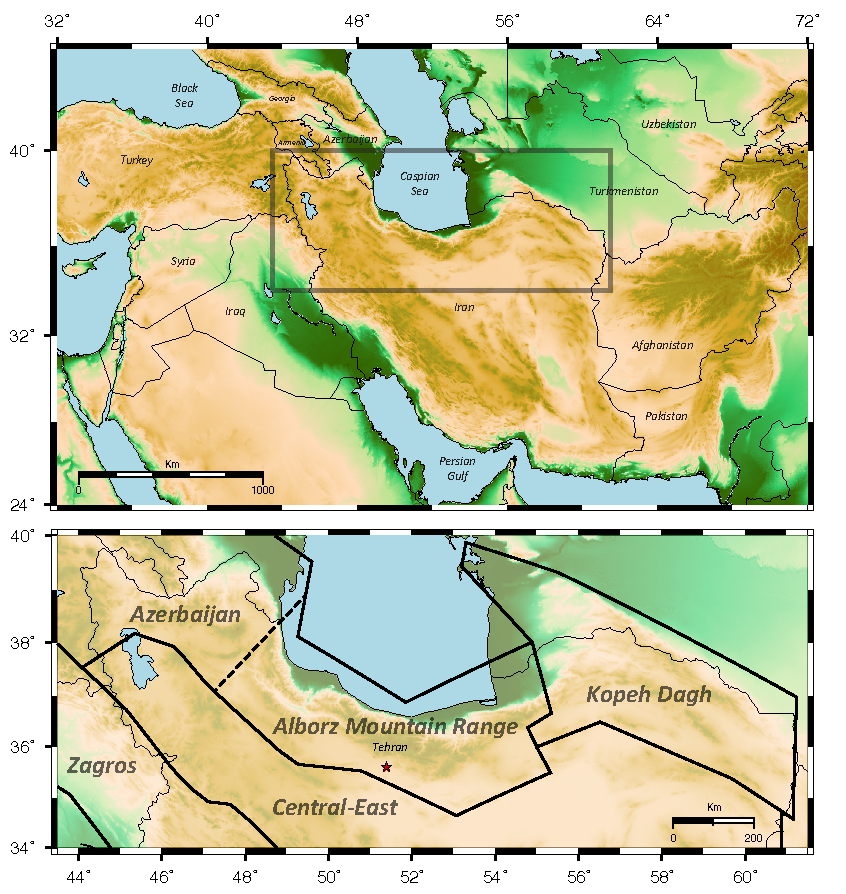
\includegraphics[width=0.8\textwidth]{figures/pdf/Figure01} 
	\caption{Sketch of the VG method. The initial events of Kopeh Dagh region are represented. Couple of events were deleted due to illustration purposes. The blue vertical lines indicate the events. Height of each line is corresponding the magnitude of the event. The green dashed lines show the allowable connections between events. The connectivity degree (K) of each event is presented. The red arrows show the time difference between events. The $T_c$ and $< T_c >$ values of the last event are represented. Note that the mean of all $<T_c>$ values in each window will be the window mean interval connectivity time.}
	\label{fig:vg}
\end{figure*}

Plotting $k$ against magnitude results on a scattered set of points which have been shown to be acceptably represented by a linear correlation, here referred to as the $k$-$M$ relationship, the slope of which also shows a linear relationship with the seismicity $b$-value of the seismic zone under consideration, or a universal sample of $k$-$M$ slope and $b$ values \citep{Telesca2013, Telesca2014}. \citet{Telesca2014} also observed that it was reasonable to draw a relationship between the distribution of the events when considering whether these were connected (visible to each other) or not and time. Let $T_c$ be the interval connectivity time, which is nothing but the time difference between two inter-visible events (see Fig.~\ref{fig:vg}); and <$T_c^e$> be the average of all $T_c$ values computed for event $e$; then it is possible to compute the visibility graph mean interval connectivity time <$T_c$>, which is the mean value of all <$T_c^e$> in a given time sequence of events.

Because <$T_c$> can be obtained for any sub-graph within a larger graph, that is, for any time window in a larger magnitude-time series of events, then it is possible to investigate the evolution of <$T_c$> (and that of the $k$-$M$ slope and the $b$-value) for a moving window sliding along the magnitude-time series. When doing so, \citet{Telesca2014} suggested to associate the values of each sub-sequence with the last event in the sequence. Following this approach, \citet{Telesca2014, Telesca2016} found that the variation of <$T_c$> over time exhibited a possible relationship with the occurrence of earthquakes. This and the aforementioned relationship between the $k$-$M$ slope and the $b$-value are aspects we explore next for our region and earthquake-sequence of interest.

% Fig.~\ref{fig:vg} shows initial events of KopehDagh magnitude-time series with connectivity degree of each event. 

